\subsection{Random variables : {\tt random\_variable\index{random\_variable} randvar\index{randvar}}}

{\tt randvar} (alias: {\tt random\_variable}) takes a probability distribution specification as its argument and returns an object representing a random variable. Its value(s) can be generated subsequently by calling {\tt sample}, {\tt rand}, {\tt randvector} or {\tt randmatrix}.

The probability distribution is specified as a sequence of arguments. The supported types are : uniform, normal, binomial, multinomial, negbinomial, Poisson, Student, Fisher-Snedecor, Cauchy, Weibull, beta, gamma, chi-square, geometric, exponential and discrete.

\paragraph{Continuous distributions.} The usual way to specify a continuous distribution is to pass the probability density function as the first argument, followed by one or more (numeric) parameters. However, it can also be defined by specifying its type and first and/or second moment (the mean and/or the standard deviation/variance); the supported types are : normal, uniform, binomial, Poisson, geometric, exponential, gamma, beta and Weibull. Additionally, a uniform distribution can be defined by specifying its range as an interval. The arguments are entered in form:
\begin{itemize}
  \item {\tt mean=}$\mu$
  \item {\tt stddev=}$\sigma$
  \item {\tt variance=}$\sigma^2$
  \item {\tt [range=]a..b} or {\tt range=[a,b]}
\end{itemize}

\paragraph{Discrete distributions.} To create a discrete random variable one can pass either
\begin{itemize}
  \item a list $W=[w_1,w_2,\dots,w_n]$ of nonnegative weights as the first argument, optionally followed by a list of values $V=[v_1,v_2,\dots,v_n]$,
  \item a list of of object-weight pairs : $[[v_1,w_1],[v_2,w_2],\dots,[v_n,w_n]]$, or
  \item a nonnegative function $f$ followed by a range specification {\tt [range=]a..b} and optionally either a positive integer $N$ (with $a,b\in\mathbb{R}$) or a list of values $V=[v_0,v_1,v_2,\dots,v_n]$ where $n=b-a$, $a<b$ and $a,b\in\mathbb{Z}$.
\end{itemize}
The weights are automatically scaled by the inverse of their sum to obtain the values of the probability mass function. If a function $f$ is given instead of a list of weights, then $w_k=f(a+k)$ for $k=0,1,\dots,b-a$ unless $N$ is given, in which case $w_k=f(x_k)$ where $x_k=a+(k-1)\,\frac{b-a}{N}$ and $k=1,2,\dots,N$. The resulting random variable $X$ has values in $\{0,1,\dots,n-1\}$ for 0-based modes (e.g.~Xcas) resp.~in $\{1,2\dots,n\}$ for 1-based modes (e.g.~Maple). If the list $V$ of custom objects is given, then $V[X]$ is returned instead of $X$. If $N$ is given, then $v_k=x_k$ for $k=1,2,\dots,N$.

\paragraph{Examples.} To define a random variable with a Fisher-Snedecor distribution (two degrees of freedom), input :
\begin{center}
  \tt X:=random\_variable(fisher,2,3)
\end{center}
Output :
\begin{center}
  \tt fisherd(2,3)
\end{center}
To generate some values of $X$, input :
\begin{center}
  \tt rand(X) // alternative : sample(X)
\end{center}
Output :
\begin{center}
  \tt 2.0457
\end{center}
Input :
\begin{center}
  \tt randvector(5,X) // alternative : sample(X,5)
\end{center}
Output :
\begin{center}
  \tt [3.9823,0.50771,0.44836,0.79225,0.088813]
\end{center}
To define a random variable with multinomial distribution, input :
\begin{center}
  \tt M:=randvar(multinomial,[1/2,1/3,1/6],[a,b,c])
\end{center}
Output :
\begin{center}
  \tt 'multinomial',[1/2,1/3,1/6],[a,b,c]
\end{center}
Input :
\begin{center}
  \tt randvector(10,M)
\end{center}
Output :
\begin{center}
  \tt [a,c,b,a,b,b,a,b,b,b]
\end{center}
Some continuous distributions can be defined by specifying its first and/or second moment. Input :
\begin{center}
  \tt randvector(10,randvar(poisson,mean=5))
\end{center}
Output :
\begin{center}
  \tt [5,4,4,8,3,8,3,3,5,9]
\end{center}
Input :
\begin{center}
  \tt randvector(5,randvar(weibull,mean=5.0,stddev=1.5))
\end{center}
Output :
\begin{center}
  \tt [3.6483,3.4194,6.8166,4.3778,2.4178]
\end{center}
Input :
\begin{center}
  \tt X:=randvar(binomial,mean=18,stddev=4)
\end{center}
Output :
\begin{center}
  \tt binomial(162,1/9)
\end{center}
Input :
\begin{center}
  \tt X:=randvar(weibull,mean=12.5,variance=1)
\end{center}
Output :
\begin{center}
  \tt weibulld(3.0857,13.98)
\end{center}
Input :
\begin{center}
  \tt mean(randvector(1000,X))
\end{center}
Output :
\begin{center}
  \tt 12.582
\end{center}
Input :
\begin{center}
  \tt G:=randvar(geometric,stddev=2.5)
\end{center}
Output :
\begin{center}
  \tt geometric(0.32792)
\end{center}
Input :
\begin{center}
  \tt evalf(stddev(randvector(1000,G)))
\end{center}
Output :
\begin{center}
  \tt 2.4245
\end{center}
Input :
\begin{center}
  \tt randvar(gammad,mean=12,variance=4)
\end{center}
Output :
\begin{center}
  \tt gammad(36,3)
\end{center}
Uniformly distributed random variables can be defined by specifying the support as an interval. Input :
\begin{center}
  \tt randvector(5,randvar(uniform,range=15..81))
\end{center}
Output :
\begin{center}
  \tt [61.97,76.427,37.939,69.639,40.325]
\end{center}
Input :
\begin{center}
  \tt rand(randvar(uniform,e..pi))
\end{center}
Output :
\begin{center}
  \tt 3.0434
\end{center}
The following examples demonstrate various ways to define a discrete random variable. Input :
\begin{center}
  \tt X:=randvar([["apple",1/3],["orange",1/4], ["pear",1/5],["plum",13/60]]):;\\randvector(5,X)
\end{center}
Output :
\begin{center}
  \tt ["apple","plum","pear","orange","apple","pear"]
\end{center}
Input :
\begin{center}
  \tt W:=[1,4,5,3,1,1,1,2]:; X:=randvar(W):;\\approx(W/sum(W))
\end{center}
Output :
\begin{center}
  \tt [0.055556,0.22222,0.27778,0.16667, 0.055556,0.055556,0.055556,0.11111]
\end{center}
Input :
\begin{center}
  \tt frequencies(randvector(10000,X))
\end{center}
Output :
\begin{center}
  \tt [[0,0.0566],[1,0.2152],[2,0.2798],[3,0.1683], [4,0.0594],[5,0.0564],[6,0.0568],[7,0.1075]]
\end{center}
Input :
\begin{center}
  \tt X:=randvar(k->1-(k/10)\verb|^|2,range=-10..10):;\\histogram(randvector(10000,X),-10,0.33,display=filled)
\end{center}
Output :
\begin{center}
  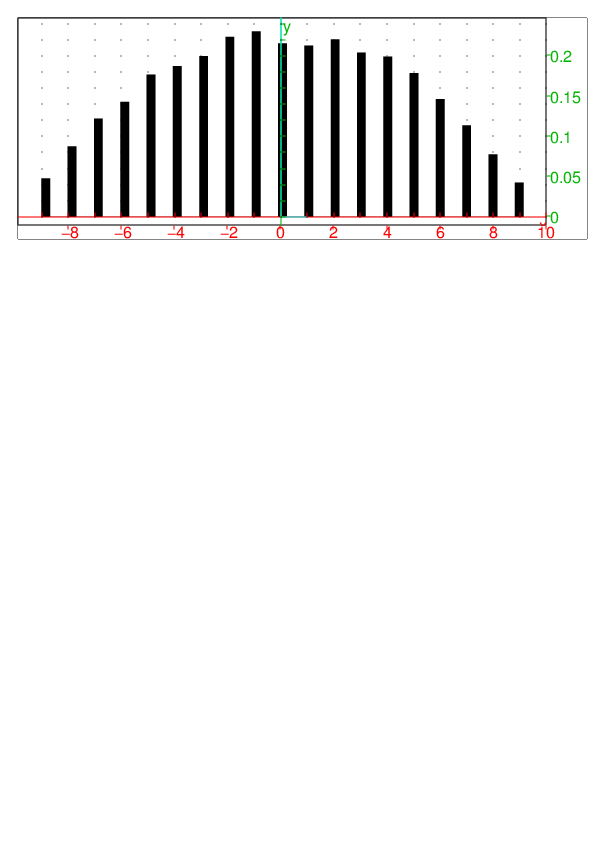
\includegraphics[width=0.75\textwidth]{random_hist1.png}
\end{center}
Input :
\begin{center}
  \tt X:=randvar([3,1,2,5],[alpha,beta,gamma,delta]):;\\randmatrix(5,4,X)
\end{center}
Output :
\[ \begin{vmatrix}\alpha&\beta&\delta&\delta\\ \delta&\alpha&\alpha&\alpha\\ \delta&\gamma&\alpha&\delta\\
\delta&\alpha&\delta&\alpha\\ \alpha&\beta&\delta&\delta\end{vmatrix}\]
Discrete random variables can be used to approximate custom continuous random variables. For example, consider a probability density function $f$ as a mixture of two normal distributions on the support $S=[-10,10]$. We sample $f$ in $N=10000$ points in $S$. Input :
\begin{center}
  \tt F:=normald(3,2,x)+normald(-5,1,x):; c:=integrate(F,x=-10..10):;\\
  f:=unapply(1/c*F,x):;\\
  X:=randvar(f,range=-10..10,10000):;
\end{center}
Now we generate 25000 values of $X$ and plot a histogram :
\begin{center}
  \tt R:=sample(X,25000):;\\
  hist:=histogram(R,-10,0.1):;\\
  PDF:=plot(f(x),display=red+line\_width\_2):;
  hist,PDF
\end{center}
Output :
\begin{center}
  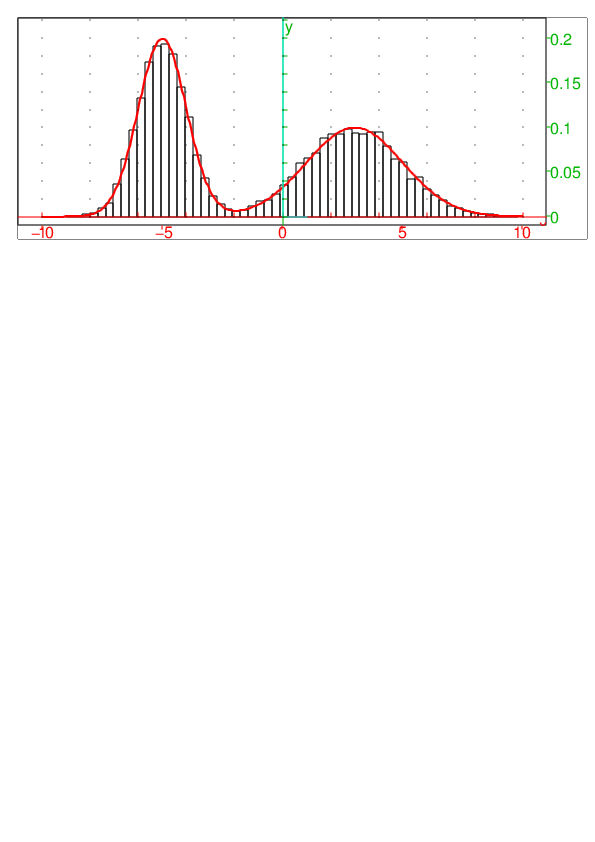
\includegraphics[width=0.75\textwidth]{random_hist2.png}
\end{center}
Sampling from discrete distributions is fast : generating 25 million samples from the distribution of X which
has about 10000 outcomes takes only couple of seconds. In fact, the sampling complexity is constant.
Also observe that the process isn't slowed down by spreading it across 1000 calls of randvector. Input :
\begin{center}
  \tt for k from 1 to 1000 do randvector(25000,X); od:;
\end{center}
{\tt Evaluation time: 2.12}

Independent random variables can be combined in an expression, yielding a new random variable.
In the example below, we define a log-normally distributed variable Y from a variable X with standard
normal distribution. Input :
\begin{center}
  \tt X:=randvar(normal):; mu,sigma:=1.0,0.5:;\\Y:=exp(mu+sigma*X):;\\L:=randvector(10000,Y):; histogram(L,0,0.33)
\end{center}
Output :
\begin{center}
  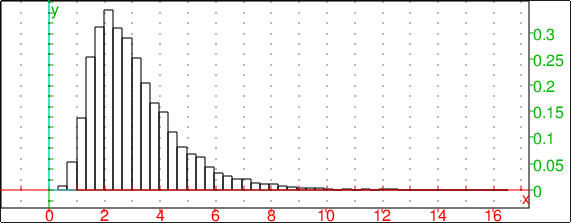
\includegraphics[width=0.75\textwidth]{random_hist3.png}
\end{center}
It is known that $E[Y]=\mathrm{e}^{\mu+\sigma^2/2}$. The mean of $L$ should be close to that number. Input :
\begin{center}
  \tt mean(L); exp(mu+sigma\verb|^|2/2)
\end{center}
Output:
\begin{center}
  \tt 3.0789,3.0802
\end{center}

In case a compound random variable is defined as an expression containing several independent random variables $X,Y,\dots$ of the same type, it is sometimes needed to prevent its evaluation when passing it to {\tt randvector} or {\tt randmatrix}. Input :
\begin{center}
  \tt Y:=randvar(normal):;
\end{center}
$X/Y$ is wrapped by eval because otherwise it would automatically reduce to 1 as $X$ and $Y$ are both {\tt normald}$(0,1)$. Input :
\begin{center}
  \tt randvector(5,eval(X/Y,0))
\end{center}
Output :
\begin{center}
  \tt [0.2608,-0.056913,-4.7966,-1.2622,-1.2997]
\end{center}
To save typing, one can define Z with {\tt eval}$(\ast,0)$ and pass {\tt eval}$(Z,1)$ to {\tt randvector} or {\tt randmatrix}. Input :
\begin{center}
  \tt Z:=eval(X/Y,0):; randvector(5,eval(Z,1))
\end{center}
Output :
\begin{center}
  \tt [0.19015,-2.4509,-1.4277,-1.1452,1.2935]
\end{center}
Parameters of a distribution can be entered as symbols to allow (re)assigning them at any time. Input :
\begin{center}
  \tt purge(lambda):; X:=randvar(exp,lambda):;\\lambda:=1:;
\end{center}
Now execute the following command line several times in a row. The parameter $\lambda$ is updated in each iteration :
\begin{center}
  \tt r:=rand(X); lambda:=sqrt(r)
\end{center}
Output (by executing the above command line three times) :
\begin{center}
  \tt 8.5682,2.9272\\1.5702,1.2531\\0.53244,0.72968
\end{center}
